\documentclass[12pt, twoside]{book} % 12 pt font, two-sided book style
\usepackage[a4paper, includehead, headheight=0.6cm, inner=3cm ,outer=2.5cm, top=2.5 cm, bottom=2.5cm]{geometry}  % Changing size of document
\usepackage[english]{babel} % The document is in English
\usepackage[utf8]{inputenc} % UTF8 encoding
\usepackage[T1]{fontenc} % Font encoding

\usepackage{graphicx} % For including images
\graphicspath{{./Images/}} % Specifies the directory where pictures are stored
\usepackage{longtable} % tables that can span several pages
\usepackage[bf]{caption} % caption: FIG in bold
\usepackage{fancyhdr} % For the headers

\newcommand{\numberedchapter}{ % Preparation for numbered chapters
	\cleardoublepage % To make sure the previous headers are passed
	\fancyhead[RE]{{\bfseries \leftmark}}% Headers for left pages
	\fancyhead[LO]{{\bfseries \rightmark}}}% Headers for right pages
\newcommand{\unnumberedchapter}[1]{ % Preparation for unnumbered chapters
	\cleardoublepage % To make sure the previous headers are passed
	\addcontentsline{toc}{chapter}{#1} % Also adds the chapter name to the Contents
	\fancyhead[RE]{{\bfseries #1}} % Headers for left pages
	\fancyhead[LO]{}}%Headers for right pages

\usepackage{emptypage} % No headers on an empty page

\usepackage{eso-pic} % For the background picture on the title page

\usepackage{hyperref} % Adds clickable links at references
\usepackage{longtable}
\usepackage{pdflscape}
\usepackage{array}
\usepackage{colortbl}

%----------------------------------------------------------------------------------------
%	ADD YOUR CUSTOM VALUES, COMMANDS AND PACKAGES
%----------------------------------------------------------------------------------------

% Open Preamble/mydefinitions.tex and enter some values (name, thesis title...) 
% and include your own custom LaTeX functions and packages

%----------------------------------------------------------------------------------------
%	VALUES FOR THE THESIS
%----------------------------------------------------------------------------------------

\newcommand{\name}{Eric Raphael Huiza Pereyra} % Author name
\newcommand{\thesistitle}{Self supervised intelligent user experiences for an improved human computer interaction applied to Peruvian deaf population} % Title of the thesis
\newcommand{\submissiondate}{February, 2021} % Submission date "Month, year"
\newcommand{\supervisor}{César Armando Beltrán Castañon} % Supervisor name
%\newcommand{\cosupervisor}{C.~O'Supervisor} % Co-Supervisor name, comment this line if there is none%


%----------------------------------------------------------------------------------------
%	BIBLIOGRAPHY STYLE (pick the style you want)
%----------------------------------------------------------------------------------------

\usepackage[square, numbers, sort&compress]{natbib} % for bibliography - Square brackets, citing references with numbers, citations sorted by appearance in the text and compressed (as in [4-7])
%\usepackage[longnamesfirst,round]{natbib} % Natural Sciences bibliography

\bibliographystyle{Preamble/physics_bibstyle} % You may use a different style adapted to your field
%\bibliographystyle{unsrtnat} % You may use a different style adapted to your field


%----------------------------------------------------------------------------------------
%	YOUR PACKAGES (be careful of package interaction)
%----------------------------------------------------------------------------------------

\usepackage{amsthm,amsmath,amssymb,amsfonts,bbm}% Math symbols

%----------------------------------------------------------------------------------------
%	YOUR DEFINITIONS AND COMMANDS
%----------------------------------------------------------------------------------------

% New Commands
\newcommand{\bea}{\begin{eqnarray}} % Shortcut for equation arrays
\newcommand{\eea}{\end{eqnarray}}
\newcommand{\e}[1]{\times 10^{#1}}  % Powers of 10 notation

% Defining a theorem box for Criteria
\newtheorem{critere}{Criterion}
\newcommand{\crit}[2]{
\begin{center}  
\fbox{ \begin{minipage}[c]{0.9 \textwidth}
\begin{critere}
\textbf{\textup{ #1}} --- #2
\end{critere}
\end{minipage}  } \end{center}
}

\begin{document}

%----------------------------------------------------------------------------------------
%	TITLE PAGE
%----------------------------------------------------------------------------------------

\pagestyle{empty} % No page numbers
\frontmatter % Use roman page numbering style (i, ii, iii, iv...) for the preamble pages

\begin{titlepage}
\begin{center}
\vfill
{\large \scshape Pontifical Catholic University of Peru\\Postgraduate School}\\[1.4cm]
{\Large Doctoral Thesis Proposal}\\[0.5cm]
\rule{\textwidth}{1.5pt}\\[0cm]
{\huge \bfseries \thesistitle \par \ }\\[-0.5cm]
\rule{\textwidth}{1.5pt}\\[2.5cm]
by\\[1cm]
{\large \bfseries\name}\\[2cm]
Supervisor\\[1cm]
{\large \textbf{\supervisor}} \\ 
\vfill
%\ifx\cosupervisor\undefined\else{\hfill \large Co-Supervisor: \textbf{\cosupervisor}} \\ \fi%
\vspace{1cm}
\submissiondate
\end{center}
\end{titlepage}

%----------------------------------------------------------------------------------------
%	PREAMBLE PAGES (comment out unnecessary pages)
%----------------------------------------------------------------------------------------

\pagestyle{fancy} % Changes the headers
\renewcommand{\chaptermark}[1]{ \markboth{#1}{}} % Getting the chapter name right
\renewcommand{\sectionmark}[1]{\markright{\thesection\; #1}} % Getting the section name right
\fancyhf{}% Clears header and footer
\fancyhead[RO,LE]{\thepage} % page number on the outside of headers

\unnumberedchapter{Abstract} 
\chapter*{Abstract} 
\subsection*{\thesistitle}

People with temporal or permanent disabilities who aim to interact with computer based system faces a series of difficulties finding technology that fit their needs. Deafness is known to be the most prevalent disability in the Peruvian population who represents a minority with no equal access to technology and services. 

Recent advances in user experience, usability standards and regulations supported the emergence of inclusive computer systems. However very little has been done to enable user experiences specialized for deaf. This doctoral thesis proposal describes a future effort that combines state of art self supervised learning techniques for unlabeled corpus annotation,  graphical gestural user interfaces to implement functional prototype user interface that enables a fluent communication between deaf and a computing system.

Self supervised learning techniques will be applied to the Peruvian signs language corpus developed by the grammar and signs research group of the Pontifical Catholic University of Peru contributing with future researches on the Signs Language recognition field. Human modeling animation will be applied to the self supervised annotation output for building the graphical gestural user interface.

We believe this work will tremendously contribute with the scientific community specially with the Peruvian community who is actively working on improving and enabling technology access to minorities.

%----------------------------------------------------------------------------------------
%	LIST OF CONTENTS/FIGURES/TABLES
%----------------------------------------------------------------------------------------

\unnumberedchapter{Contents}
\tableofcontents % Write out the Table of Contents

%----------------------------------------------------------------------------------------
%	THESIS MAIN TEXT - CHAPTERS
%----------------------------------------------------------------------------------------

\addtocontents{toc}{\vspace{2em}} % Add a gap in the Contents, for aesthetics
\mainmatter % Begin numeric (1,2,3...) page numbering

\numberedchapter

\chapter{Introduction and planning} \label{ch-1}

\section{Introduction}

The World Health Organization (WHO) stated that 466 million people worldwide have disabling hearing loss posing a global cost of 750 million dollars annually for unaddressed cases, estimating that by 2050 over 900 million people will have this condition. Current estimates suggest 83\% gap in hearing aid needed and use i.e., only 17\% of those who could benefit from using some kind of hearing aid\cite{deafness_and_hearing_loss_2020}, configuring a real need for investing on inclusive computing system that help on decreasing the gap and enable people with the tools to successfully interact with computer systems.

The Peruvian Institute of Informatics and Statistics (INEI) conducted a national disabilities survey with the objective of developing a better understanding about disabilities that affect the Peruvian population as well as their prevalence and posterior segmentation\cite{disabilities_survey_2012}. Results showed that 1.8\% of the Peruvian population suffer at least partially when not permanent deafness or hearing limitations indicating that approximately half a million people in the country is subject to have impediments or difficulties while performing day to day tasks that require the assistance of computer based systems. Peruvians with deafness or hearing limitations use the Peruvian Signs Language (PSL) as their main communication medium. PSL is mandatory at universities and certain public institutions as well as some official acts but is not common or nonexistent in the majority of venues and acts, henceforth the importance of designing systems that are capable to synthesize PSL inputs and simulate or generate PSL compatible outputs in a natural way. Furthermore, it is worth to indicate that in the same way as spoken languages, signs languages present local variations i.e. people living in Lima metropolitan area are not expected to use the same set of signs as people in other parts of the territory thereby it is correct to assume the existence of local PSL variations that enrich the language but at the same time add complexity towards to standardization, description and processing. This work will use a dataset containing PSL recordings with the variation used in the Lima metropolitan area due to the difficulty or inability to find datasets for other PSL variations.

The Grammar and Signs research group of the Pontifical Catholic University of Peru (PUCP) built the first PSL dataset  which is publicly available at the university digital archives. The dataset consists of a set of recordings following a method that involves a signer, a translator and a coordinator. It is important to highlight that the dataset is neither labeled or annotated and cannot be used as it is for training or testing a machine learning model. This work elaborates a method for extracting features and learning PSL elements using a self supervised approach.

A grammatically description of the PSL elements including but not limited to phonology, dactylology, numbers, common expressions, gender, verb tenses, question forms, nouns and adjectives then continued with a definition of PSL manual and non manual features where manual features refers to hand gestures and non manual refers to other body parts sections like neck, shoulders and the head. It is important to establish the relation between grammatical rules and manual or non manual features for which we will use the HamNoSys / SiGML notation in the context of an isolated signs detection method which is then extended to a continuous signs detection method approached as a self supervised learning task focused on learning features from the PSL dataset using representational autoencoders and energy functions (LeCun et al. 2020) while reconstructing PSL elements.

A conversational user interface between deaf and a computing system enabled by a graphical gestural user interface powered by HAmin for a 3D human simulation achieved by synthesizing PSL to Spanish and then Spanish to a PSL bundled into a mobile application that can be installed as a standalone application or an extension to existing application or services.

This doctoral project pursues the main objective of building "A novel solution for deaf users who aim to improve their human-computer interaction enabled by state of art self supervised learning and computer vision methods." and the following specific objectives:

\begin{itemize}
\item Produce an efficient self supervised method for annotating small non annotated signs language datasets applied to the Peruvian signs language corpus produced by the Grammar and Signs research group of the Pontifical Catholic University of Peru generalizable to other sign languages datasets.
\item Produce a Nielsen heuristics aware graphical gestural user interface capable of enabling an effective bidirectional human computer interaction between deaf users and a device powered by an algorithm trained with the dataset produced in the objective above.
\item Produce a prototype installable and distributable application powered by the algorithm and user interface produced in objectives 1 and 2.
\end{itemize}


The rest of the document is organized as follows. In section \ref{literature-review} we review the related work and state-of-art on sign languages recognition, self supervised learning applied to images and videos and graphical gestural user interfaces. In sections \ref{research-schedule} and \ref{research-budget} we describe the schedule and budget plan for executing the set of tasks needed to complete the doctoral project and finally in section \ref{available-datasets} we present the available datasets for signs language recognition and their details.


\section{Literature Review}\label{literature-review}
\subsection{Signs Language Recognition and annotation}
Signs Language Recognition (SLR) are roughly divided in two categories Isolated SLR and Continuous SLR\cite{adaloglou2020comprehensive} figure \ref{fig-slr} shows tasks involved on SLR.

\subsubsection{Isolated Signs Language Recognition}
Methods using this approach will assume individual and well defined glosses that are recognized in a series of video frames. Recognizing gestures is a difficult task, due to intrapersonal and interpersonal variations in performing them. In \cite{kennaway2015avatar} a new descriptive language called SiGML (Signing Gesture Markup Language) is presented, SiGML was developed from HamNoSys, the Hamburg Notation System. HamNoSys is a notation for recording sign language gestures, developed by researchers on sign language at the IDGS (Institut für Deutsche Ge-bädensprache) at the University of Hamburg, it is not specific to any one sign language, but is intended to cover all signing gestures in all sign languages. It records sign languages elements in terms of hand shape, hand location and hand movement and other special terms for non manual gestures. Signs are not holistic gestures but are rather analyzable, as a combination of linguistically significant features. Similarly to spoken languages, Signs Languages are composed of the following indivisible features\cite{adaloglou2020comprehensive}:
\begin{itemize}
\item Manual features, i.e. hand shape, position, movement, orientation of the palm or fingers
\item Non-manual features, namely eye gaze, head-nods/ shakes, shoulder orientations, various kinds of facial expression as mouthing and mouth gestures.
\end{itemize}
SiGML provides a formal notation that is easily understood by computer because it is XML based as shown in the figure \ref{fig-sigml}.

\subsubsection{Continuous Signs Language Recognition}
Continuous Signs Language Recognition (CSLR) uses contextual information that is not limited to spatial information that resides around the hand shape for fixed point in time, but also temporal information that consists of hand and body movements. Signs are famously multi-channel, information is carried in the hand shape, motions, body pose and even facial gestures \cite{slimane2021context}, \cite{camgoz2017subunets}. While models that recognize text based language use punctuation marks to separate sentences, CSLR models use pauses e.g. silent regions. There have been studies in the literature addressing automatic sign segmentation. However to the best of the authors’ knowledge, there is no study which utilizes sign segmentation for realizing continuous sign language recognition for complex scenarios. Following successful segmentation, the system needs to under-stand what information is being conveyed within a sign sentence. Current approaches tackle this by recognizing sign glosses and other linguistic components. Such methods can be grouped under the banner of CSLR. From a computer vision perspective, this is the most challenging task. Considering the input of the system is high dimensional spatio-temporal data, i.e. sign videos, models are required that understand what a signer looks like and how they interact and move within their 3D signing space. Moreover, the model needs to comprehend what these aspects mean in combination. This complex modeling problem is exacerbated by the asynchronous multi-articulatory nature of sign languages. Although there have been promising results towards CSLR, the state-of-the-art can only recognize sign glosses and operate within a limited domain of discourse, namely weather forecasts \cite{camgoz2020sign}

\subsubsection{Sign Languages Recognition Approaches}
\textbf{Specialized sub-networks (SubUNets)} allow decomposing a complex signs recognition problem into a series of specialized expert systems allowing to learn both spatial and temporal features where each subunit learns an intermediate representation that is transferred to the next subunit. (Camgoz et al.) \cite{camgoz2017subunets} proposed an architecture where each SubUNet consists of three tiers, firstly Convolutional Neural Network layer to learn spatial features, then a Bidirectional Long Short Term Memory layer to learn temporal features on top of the spatial features and finally a Connectionist Temporal Classification Loos layer to allow the networks to be trained with different length videos and label sequences as presented in figure \ref{temporal-modeling}. (Huang et al.) \cite{huang2018videobased} proposed a two streams \textbf{3DCNN} architecture for learning global (entire video frame) and local (hands area crop) video representations in combination with a Hierarchical Attention Network (HAN) for latent space based recognition eliminating the need for temporal layers as proposed in other studies \cite{slimane2021context}, \cite{camgoz2017subunets}, \cite{camgoz2020sign}. HAN is an extension of LSTM which incorporates the attention mechanism based on the structure of input. It uses a latent space which maps video representations learned on the 3DCNN streams with relevant video sentences using one hot encoding vectors. The encoder in the HAN reflects the hierarchical structures in its inputs and incorporates the attention mechanism.

\subsection{Graphical Gestural User Interfaces}
A subset of Natural Language Processing called natural language generation or simply generation produces sentences from semantic information. The lack of a written form for most sign languages means that these traditional processing stages work somewhat differently. Instead of a written string, many sign language systems will create some type of script (generally in a proprietary format for each system) that specifies the movements for an animated character. Instead of speech output, sign language systems produce an animation of a humanlike character performing the sentence (based on the information encoded in the script) \cite{huenerfauth2009sign}. HamNoSys defines a notation which is independent of the Signs Languages. A HamNoSys transcription is independent of the person or avatar performing it which solves the problem of different signers styles while signing. It records only those aspects of the gesture which are significant for the correct performance of a sign. HamNoSys defines a Signing space, see figure \ref{fig-signing-space} and a set of pre-defined locations see figure \ref{fig-signing-locations} on the surface of the body figures \cite{kennaway2015avatar}

To generate motion data for a particular avatar, numerical information about the avatar must be supplied, to be combined with the avatar- independent description of the movement, to produce avatar-specific motion data. The information required divides into two classes, information about the geometry of a specific avatar, and information about body language or signing style, which can vary independently of the avatar.
The geometrical information required about the avatar consists of:
\begin{itemize}
\item The dimensions of the avatar’s skeleton: the lengths of its bones, and the positions and orientations of the bones in some standard posture.
\item For each of the non-manuals defined in HamNoSys, the mixture of avatar-specific facial morphs or bone rotations which implements it.
\item The coordinates of every location nameable in HamNoSys, relative to the bone which moves the relevant body part. In principle, a HamNoSys location should be considered as a volume having a certain extent, the choice of which point within that volume to use being dependent on the context, but for implementation we have preferred to model each location by a single fixed point.
\end{itemize}

The first of these can in principle be read automatically from whatever avatar description file is exported by the modeling software used to create it. The second requires the avatar creator to express each of the HamNoSys facial movements as a combination of the avatar’s morphs. The third requires the avatar creator to specify the coordinates of all the HamNoSys locations on the surface of the body. Some of these locations can be discovered automatically. For example, it is fairly easy to determine surface points on the palmar, dorsal, ulnar, and radial sides of each finger, level with the midpoint of the middle phalanx. Other points are best placed manually: it is easier for the modeler to say where the ears are than to determine them algorithmically from analysis of the surface mesh. Specifying the locations of these surface points should be considered a necessary part of the construction of any avatar intended for synthetic animation. Note that no other knowledge is required of the surface mesh itself, which may be arbitrarily dense, subject to the requirement of rendering it at the desired frame rate.

The “body language” class of information consists of the mapping of HamNoSys categories to numbers. It requires:
\begin{itemize}
\item A numerical definition of the size of a “large”, “medium”, or “small” movement, “near” and “far” proximities, the shape of a “deep” or “shallow” curved arc, and similarly for all the other geometric categories in HamNoSys. Distances are best given as proportions of various measurements of the avatar: for example, “far” from the chest might be defined as a certain proportion of the length of either arm.
\item A numerical specification of the time required for each type of movement, and of how that time should change when HamNoSys specifies the manner of movement as “fast”, “slow”, “tense”, etc.
\item A numerical specification of how the hands should accelerate and decelerate during movements of different types, performed with different manners.
\item The temporal trajectories that the avatar-specific morphs and bone rotations that implement non-manual movements should follow. This takes the form of attack, sustain, and release times, plus a description of how the elements of the movement ramp up from zero to the full value during the attack, and down again to zero during the release.
\end{itemize}

Body language information is specific, not to a particular avatar body, but to the personality inhabiting it. Given all of this information, generating motion data requires solving the following problems \cite{kennaway2015avatar}.

\section{Research Schedule}\label{research-schedule}
\begingroup
\footnotesize
\begin{longtable}{|>{\hspace{0pt}}m{0.042\linewidth}|>{\hspace{0pt}}m{0.311\linewidth}|>{\hspace{0pt}}m{0.388\linewidth}|>{\centering\hspace{0pt}}m{0.096\linewidth}|>{\centering\arraybackslash\hspace{0pt}}m{0.096\linewidth}|} 
\hline
\rowcolor[rgb]{0.502,0.502,0.502}  & \multicolumn{1}{>{\centering\hspace{0pt}}m{0.311\linewidth}|}{TASK\textbf{}} & \multicolumn{1}{>{\centering\hspace{0pt}}m{0.388\linewidth}|}{DESCRIPTION} & START \par{}DATE & END \par{}DATE \endfirsthead 
\hline
\rowcolor[rgb]{0.753,0.753,0.753} 1 & SELF SUPERVISED CORPUS \par{}ANNOTATION & DESIGN AND IMPLEMENT A SELF \par{}SUPERVISED PSL CORPUS \par{}ANNOTATION~METHOD & 03/15/2021 & 07/14/2022 \\ 
\hline
1.1 & Initial corpus clean up. & Perform initial corpus cleaning tasks \par{}including\par{}1. Video organization (titles, dates, \par{}duration, signer).\par{}2. Video storage in a cloud system. & 03/15/2021 & 03/26/2021 \\ 
\hline
1.2 & Peruvian sings language grammatical \par{}rules description. & Perform a detailed description of the \par{}Peruvian signs language elements \par{}including:\par\null\par{}1. Phonology.\par{}2. Dactylology.\par{}3. Numbers.\par{}4. Common Expressions.\par{}5. Vocabulary.\par{}6. Gender.\par{}7. Verb tenses.\par{}8. Question forms.\par{}9. Nouns.\par{}10. Adjectives. & 03/15/2021 & 23/07/2021 \\ 
\hline
1.3 & Define peruvian signs language \par{}manual and non manual features. & Create a descriptive list of manual \par{}and non manual features available in \par{}PSL e.g. hand shapes, rotation, \par{}orientation and other body parts like \par{}neck orientation, shoulders and arms \par{}movements. & 03/15/2021 & 03/15/2021 \\ 
\hline
1.4 & Establish relations between \par{}grammatical rules, manual and \par{}non manual features. & Using the HamNoSys / SiGML notation \par{}define the manual and non manual \par{}features for the most common \par{}PSL elements. & 03/15/2021 & 12/17/2021 \\ 
\hline
1.5 & Design the input preprocessing \par{}method. & Design the architecture design for the \par{}data input pipeline including data \par{}transformation and augmentation. \par{}The design should contain elements to \par{}detect the signer (object detection) and \par{}perform a more granular body parts \par{}detection using state of art mechanisms. & 04/19/2021 & 05/14/2021 \\ 
\hline
1.6 & Implement the input preprocessing \par{}method. & Implement the architecture designed \par{}in 1.5 and produce a software based \par{}solution for pre-processing raw PSL videos \par{}and generate a list of PSL manual and \par{}non manual elements. & 05/17/2021 & 09/10/2021 \\ 
\hline
1.7 & Design the feature extraction \par{}method. & Design a method that is capable to find \par{}relations between manual and non manual \par{}features using Word2Vec as a \par{}starting point but extended to a Visual words. & 06/07/2021 & 07/05/2021 \\ 
\hline
1.8 & Implement the feature extraction \par{}method. & Implement a software solution based on \par{}1.7 that is capable to find relations between \par{}manual and non manual features on the \par{}same glose (isolated signs detection). & 07/06/2021 & 10/11/2021 \\ 
\hline
1.9 & Design the temporal sequencing \par{}method. & Once an isolated signs detection method \par{}is implemented, extend it to a method to \par{}determine temporal sequencing between \par{}isolated signs in order to detect more complex \par{}PSL elements (e.g expressions). & 10/12/2021 & 11/12/2021 \\ 
\hline
1.10 & Implement the temporal sequencing \par{}method. & Implement a software solution that is \par{}capable to perform a continuous \par{}signs detection using temporal \par{}sequencing based on the design in 1.9. & 11/15/2021 & 12/17/2021 \\ 
\hline
1.11 & Isolated Signs Language \par{}Recognition. & Based on 1.8 create an isolated signs \par{}language dataset. & 20/12/2021 & 01/14/2022 \\ 
\hline
1.12 & Continuous Signs Language \par{}Recognition. & Based on 1.10 create a continuous signs \par{}language dataset. & 01/17/2022 & 01/31/2022 \\ 
\hline
1.13 & Design the self and continuously \par{}improving signs detection method. & Design a solution based on Energy functions \par{}and Representational Autoencoders to allow \par{}predicting and reconstructing PSL elements \par{}in order to enter into a continuous improvement \par{}executing tasks 1.5 to 1.12. & 01/02/2022 & 03/31/2022 \\ 
\hline
1.14 & Implement the self and continuously \par{}improving signs detection method. & Based on the design 1.13 implement a \par{}network architecture based on representational \par{}auto encoders with the objective to \par{}optimize an energy function. & 04/01/2022 & 07/14/2022 \\ 
\hline
1.15 & Estimate the average duration \par{}of a gloss. & Based on the design 1.13 implement a \par{}network architecture that is based on \par{}representational auto encoders and \par{}energy functions optimization to \par{}progressively detect the average \par{}duration of a PSL gloss. & 01/07/2022 & 07/14/2022 \\ 
\hline
\rowcolor[rgb]{0.753,0.753,0.753} 2 & GRAPHICAL GESTURAL USER \par{}INTERFACE & DESIGN AND IMPLEMENT A GESTURAL\par{}USER INTERFACE FOR PSL SIGNERS & \multicolumn{1}{>{\hspace{0pt}}m{0.096\linewidth}|}{07/18/2022} & \multicolumn{1}{>{\hspace{0pt}}m{0.096\linewidth}|}{07/14/2023} \\ 
\hline
2.1 & Design the conversational user \par{}interface. & Design a user interface to enable \par{}conversations between a signer and \par{}a computer. For this task we propose \par{}designing a chatbot using today’s available \par{}cloud options (e.g. Alexa) by extending it \par{}with the models implemented in 1. & \multicolumn{1}{>{\hspace{0pt}}m{0.096\linewidth}|}{07/18/2022} & \multicolumn{1}{>{\hspace{0pt}}m{0.096\linewidth}|}{08/26/2022} \\ 
\hline
2.2 & Implement the conversational user \par{}interface. & Implement the user interface designed in 2.1, \par{}it will use 3D modeling using a Human \par{}simulation approach instead of concatenating \par{}a series of videos. Human simulation modeling \par{}is achievable using current technologies like \par{}Humanoid Animation (HAmin). & \multicolumn{1}{>{\hspace{0pt}}m{0.096\linewidth}|}{08/29/2022} & \multicolumn{1}{>{\hspace{0pt}}m{0.096\linewidth}|}{11/30/2022} \\ 
\hline
2.3 & Signs Language synthesis to Spanish. & Using the algorithms approximated in 1\textbf{ }as well \par{}as the grammatical rules defined and created \par{}in 1.1, 1.2, 1.3 and 1.4 implement a software \par{}solution for synthesizing PSL elements to \par{}Spanish. & \multicolumn{1}{>{\hspace{0pt}}m{0.096\linewidth}|}{12/01/2022} & \multicolumn{1}{>{\hspace{0pt}}m{0.096\linewidth}|}{02/01/2023} \\ 
\hline
2.4 & Spanish synthesis to Signs Language. & Using the algorithms approximated in 1\textbf{ }as well \par{}as the grammatical rules defined and created \par{}in 1.1, 1.2, 1.3 and 1.4 implement a software \par{}solution for synthesizing Spanish to \par{}PSL elements. & \multicolumn{1}{>{\hspace{0pt}}m{0.096\linewidth}|}{02/01/2023} & \multicolumn{1}{>{\hspace{0pt}}m{0.096\linewidth}|}{04/01/2023} \\ 
\hline
2.5 & Signs Language Animation. & Implement the signs language animation or \par{}Human simulation modeling which is \par{}achievable using current technologies \par{}like Humanoid Animation (HAmin). & \multicolumn{1}{>{\hspace{0pt}}m{0.096\linewidth}|}{04/04/2023} & \multicolumn{1}{>{\hspace{0pt}}m{0.096\linewidth}|}{07/14/2023} \\ 
\hline
\rowcolor[rgb]{0.753,0.753,0.753} 3 & PROTOTYPE APPLICATION & DESIGN AND IMPLEMENT AN INSTALLABLE \par{}APPLICATION TO ENABLE INTERACTION\par{}BETWEEN SIGNERS AND COMPUTERS & \multicolumn{1}{>{\hspace{0pt}}m{0.096\linewidth}|}{07/17/2023} & \multicolumn{1}{>{\hspace{0pt}}m{0.096\linewidth}|}{12/15/2023} \\ 
\hline
3.1 & Design an application that can be \par{}installed in devices \par{}(e.g. mobile phones and tablets) \par{}for signers human computer \par{}interaction. & Design an iOS application that can be installed \par{}in apple devices, the application to be capable \par{}to use the set of algorithms implemented in 1 \par{}and the user gestural user interface \par{}implemented in 2. & \multicolumn{1}{>{\hspace{0pt}}m{0.096\linewidth}|}{07/17/2023} & \multicolumn{1}{>{\hspace{0pt}}m{0.096\linewidth}|}{08/21/2023} \\ 
\hline
3.2 & Implement an application that can \par{}be installed in devices and enable \par{}signers human computer interaction. & Implement an iOS application that use the \par{}design defined in 3.1. & \multicolumn{1}{>{\hspace{0pt}}m{0.096\linewidth}|}{08/22/2023} & \multicolumn{1}{>{\hspace{0pt}}m{0.096\linewidth}|}{12/15/2023} \\ 
\hline
\rowcolor[rgb]{0.753,0.753,0.753} 4 & GENERAL TASKS & COMMON GENERAL AND ADMINISTRATIVE\par{}TASKS & \multicolumn{1}{>{\hspace{0pt}}m{0.096\linewidth}|}{03/15/2021} & \multicolumn{1}{>{\hspace{0pt}}m{0.096\linewidth}|}{12/15/2023} \\ 
\hline
4.1 & Weekly meetings with thesis advisor. &  & \multicolumn{1}{>{\hspace{0pt}}m{0.096\linewidth}|}{03/15/2021} & \multicolumn{1}{>{\hspace{0pt}}m{0.096\linewidth}|}{12/12/2023} \\ 
\hline
4.2 & Weekly visits to the PUCP campus. &  & \multicolumn{1}{>{\hspace{0pt}}m{0.096\linewidth}|}{03/15/2021} & \multicolumn{1}{>{\hspace{0pt}}m{0.096\linewidth}|}{12/12/2023} \\ 
\hline
4.3 & Doctoral thesis plan. & Design and writing of the doctoral thesis plan. & \multicolumn{1}{>{\hspace{0pt}}m{0.096\linewidth}|}{03/15/2021} & \multicolumn{1}{>{\hspace{0pt}}m{0.096\linewidth}|}{07/16/2023} \\ 
\hline
4.4 & Write and publish First paper. & Write and publishing of the first paper required \par{}for the doctoral program. & \multicolumn{1}{>{\hspace{0pt}}m{0.096\linewidth}|}{08/02/2021} & \multicolumn{1}{>{\hspace{0pt}}m{0.096\linewidth}|}{07/15/2022} \\ 
\hline
4.5 & Write and publish Second paper. & Write and publishing of the second paper \par{}required for the doctoral program. & \multicolumn{1}{>{\hspace{0pt}}m{0.096\linewidth}|}{08/15/2022} & \multicolumn{1}{>{\hspace{0pt}}m{0.096\linewidth}|}{07/17/2023} \\ 
\hline
4.6 & Doctoral thesis. & Design and writing of the doctoral thesis. & \multicolumn{1}{>{\hspace{0pt}}m{0.096\linewidth}|}{03/15/2021} & \multicolumn{1}{>{\hspace{0pt}}m{0.096\linewidth}|}{12/15/2023} \\
\hline
\end{longtable}
\endgroup

\section{Research Budget}\label{research-budget}
The student counts with a USD 4000 education bonus per year provided by his employer. In the event the education bonus will not suffice the student will use his own monetary resources to cover additional expenses.
\begingroup
\footnotesize
\begin{longtable}{|>{\hspace{0pt}}m{0.286\linewidth}|>{\hspace{0pt}}m{0.357\linewidth}|>{\hspace{0pt}}m{0.104\linewidth}|>{\hspace{0pt}}m{0.19\linewidth}|} 
\hline
\rowcolor[rgb]{0.502,0.502,0.502} RESOURCES & DESCRIPTION & COST & FUNDING \endfirsthead 
\hline
\rowcolor[rgb]{0.753,0.753,0.753} SOFTWARE LICENSING &  & USD 0.00 &  \\ 
\hline
Pycharm (Student license) & IDE for python development &  &  \\ 
\hline
AppCode (Student license) & IDE for Apps development &  &  \\ 
\hline
CLion (Student license) & IDE for C and C++ development &  &  \\ 
\hline
iOS & Mobile operating system &  &  \\ 
\hline
MacOSx & Desktop operating system &  &  \\ 
\hline
TextMaker & LateX editor &  &  \\ 
\hline
\rowcolor[rgb]{0.753,0.753,0.753} CLOUD SERVICES &  & USD 5508.00 &  \\ 
\hline
AWS Sage Maker & \textcolor[rgb]{0.086,0.098,0.122}{5 jobs per month x 1 instances }\par{}\textcolor[rgb]{0.086,0.098,0.122}{per job x 8 hours per job = 40.00 }\par{}\textcolor[rgb]{0.086,0.098,0.122}{SageMaker Training hours per month}\par{}\textcolor[rgb]{0.086,0.098,0.122}{}\textcolor[rgb]{0.086,0.098,0.122}{}\par{}\textcolor[rgb]{0.086,0.098,0.122}{40.00 hours per month x 3.825 USD }\par{}\textcolor[rgb]{0.086,0.098,0.122}{per hour instance cost = 153.00 USD }\par{}\textcolor[rgb]{0.086,0.098,0.122}{(monthly On-Demand cost)}\par{}\textcolor[rgb]{0.086,0.098,0.122}{}\textbf{Total cost for SageMaker Training (monthly): }\par{}\textbf{153.00 USD}\textcolor[rgb]{0.086,0.098,0.122}{}\textcolor[rgb]{0.086,0.098,0.122}{} & USD 5508.00 & \par{}Student Education Bonus\par{}provided by employer.\par{} \\ 
\hline
GitHub & Source code versioning and control & USD 0.00 &  \\ 
\hline
S3 (Student version) & Cloud objects storage & USD 0.00 &  \\ 
\hline
Lambda / Serverless (Student version) & Functions as a service & USD 0.00 &  \\ 
\hline
\rowcolor[rgb]{0.753,0.753,0.753} PERSONEL &  & USD 0.00 &  \\ 
\hline
Doctoral student &  & USD 0.00 &  \\ 
\hline
Doctoral advisor &  & USD 0.00 &  \\ 
\hline
\end{longtable}
\endgroup

\section{Contributions}
This study will contribute with an annotated PSL dataset generalizable to other studies focused on accessibility for minorities and deaf population. Along with an annotated PSL dataset we will produce a set of state of art DNN architectures and models for learning features from a non annotated PSL dataset using self supervised techniques. The produced models will be compared using an ablative analysis focusing on indicators for Isolated Signs Language Recognition and Continuous Sign Language Recognition.  Additionally to Isolated SLR and Continuous SLR recognition models we will produce another set of state of art architectures and models for Sign Language Generation. These models will be trained to produce (regression) SiGML or HamNoSys notation from a Isolated SLR or a Continuous  SLR input. It is important to highlight that models designed for Sign Language Recognition and Sign Language Generation can be trained and used independently as building blocks for other studies in Signs Languages related tasks but at the same time can complement each other producing a pipeline that enables generating Signs Language elements from a non annotated dataset.

Finally we will animate the generated SiGML or HamNoSys Sign Language elements into a 3D animated avatar following state of art Human-Computer interaction techniques. Sign Language animation will allow closing the bridge between deaf people and computer based systems allowing a bi-directional communication and interaction.



\section{Target Indexed Journals}
\begingroup
\footnotesize
\begin{longtable}{|l|l|l|}
\caption{List of target indexed journals}\\ 
\hline
\rowcolor[rgb]{0.502,0.502,0.502} NAME & OVERVIEW & URL \endfirsthead 
\hline
\begin{tabular}[c]{@{}l@{}}International Journal \\of Machine Learning \\and Cybernetics\end{tabular} & \begin{tabular}[c]{@{}l@{}}The International Journal of Machine Learning\\~and Cybernetics (IJMLC) focuses on the key \\research problems emerging at the junction of \\machine learning and cybernetics and serves\\~as a broad forum for rapid dissemination of the \\latest advancements in the area. The emphasis \\of IJMLC is on the hybrid development of \\machine learning and cybernetics schemes \\inspired by different contributing disciplines \\such as engineering, mathematics, cognitive \\sciences, and applications. New ideas, design \\alternatives, implementations and case studies \\pertaining to all the aspects of machine learning\\~and cybernetics fall within the scope of the IJMLC.\end{tabular} & \begin{tabular}[c]{@{}l@{}}https://www.springer\\.com/journal/\\13042\end{tabular} \\ 
\hline
\begin{tabular}[c]{@{}l@{}}Machine Learning \\with Applications\end{tabular} & \begin{tabular}[c]{@{}l@{}}Machine Learning with Applications (MLWA) is a \\peer reviewed, open access journal focused on \\research related to machine learning. The journal \\encompasses all aspects of research and \\development in ML, including but not limited \\to data mining, computer vision, natural language \\processing (NLP), intelligent systems, neural networks, \\AI-based software engineering, bioinformatics and their \\applications in the areas of engineering, medicine, \\biology, education, business and social sciences. \\It covers a broad spectrum of applications in the \\community, from industry, government, and academia.\end{tabular} & \begin{tabular}[c]{@{}l@{}}https://www.journals.\\elsevier.com/\\machine-learning\\-with-applications\end{tabular} \\ 
\hline
\begin{tabular}[c]{@{}l@{}}\textcolor[rgb]{0.133,0.133,0.133}{Computers \& Electrical }\\\textcolor[rgb]{0.133,0.133,0.133}{Engineering}\end{tabular} & \begin{tabular}[c]{@{}l@{}}Published since 1973, Computers \& Electrical \\Engineering provides rapid publication of topical \\research into the integration of computer technology \\and computational techniques with electrical and \\electronic systems. The journal publishes papers \\featuring novel implementations of computers and \\computational techniques in areas like signal \\processing, high-performance computing, \\artificial intelligence, and communications.\end{tabular} & \begin{tabular}[c]{@{}l@{}}https://www.journals.\\elsevier.com/\\computers-and-\\electrical-engineering\end{tabular} \\
\hline
\end{longtable}

\endgroup % Import your chapters here
\chapter{Methodology} \label{chap-2}

\section{Available Datasets}\label{available-datasets}
The PSL dataset was developed by the PUCP Grammar and Signs research group in 2014 and consists in a set of videos recorded during the interviews of 24 individuals, 12 male and 12 female informants, all of them are Lima Peru residents and reported to be born with a permanent deafness condition or acquired the condition before the acquisition of Spanish. 

The dataset consists in 718 video clips recorded with a ADR-CX220 SONY HD camera which included an embedded microphone. The camera focused only the informant but also recorded questions, instructions and translations.

The video clips were recorded in three sessions with the following participants: A coordinator, a PSL \cite{lsp_2015} translator and a informant.\\

\textbf{Recording Session 1}: A 45-60 minutes semi structured interview that included: Biographic information as well as habits, anecdotes, opinion about cultural subjects and elicitation of names, states and actions. 

\textbf{Recording Session 2}: The informant was presented with a set of 55 cards describing actions and were asked to choose a set of them in order to build a coherent story that was subsequently told by the informant.

\textbf{Recording Session 3}: A PSL \cite{lsp_2015} conversation facilitated by the coordinator happening between the informant and the translator.

During all the sessions a PSL \cite{lsp_2015} translator performs a translation after a word or phrase is completed.

Other existing Sing Language Recognition are publicly available. These datasets can be characterized as isolated or continuous, taking into account whether annotation are provided at the gloss (fine-grained) or the sentence (coarse-grained) levels. Additionally, they can be divided into Signer Dependent (SD) and Signer Independent (SI) ones, based on the defined evaluation scheme. In particular, in the SI datasets a signer cannot be present in both the training and the test set. In Table \ref{tab:public-large-datasets}, the following most widely known public SLR datasets, along with their main characteristics.

\pagestyle{plain}
\chapter{Figures, tables and images} \label{chap-2}

\section{Figures}

\begin{figure}[hbt!]
\center
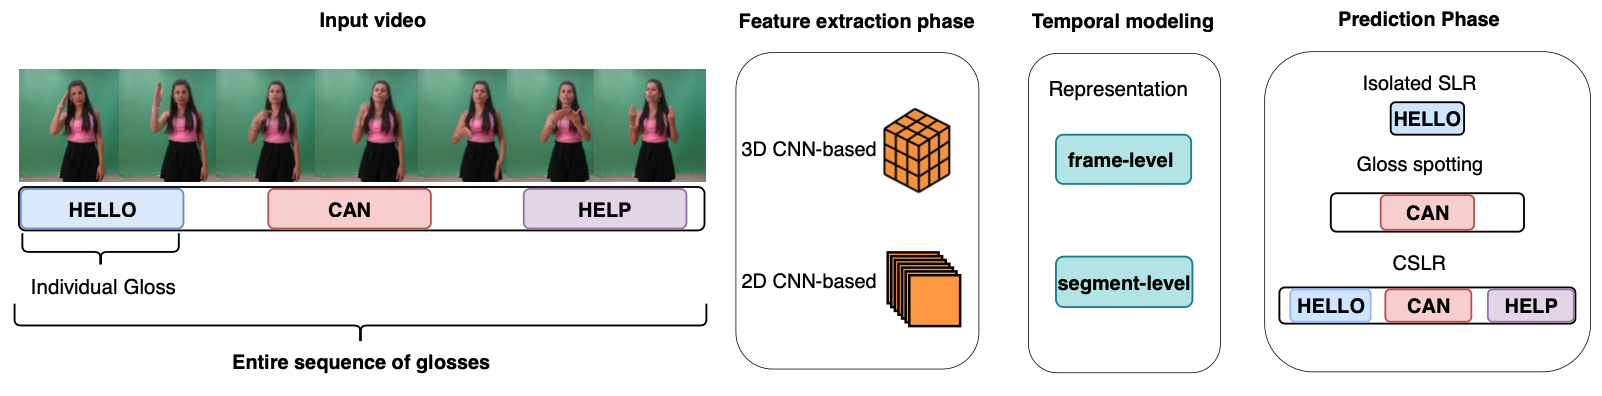
\includegraphics[width=\linewidth]{chap3/signs-language-recognition.png} 
\caption{Signs Language Recognition}
\label{fig-slr}
\end{figure}

\begin{figure}[hbt!]
\center
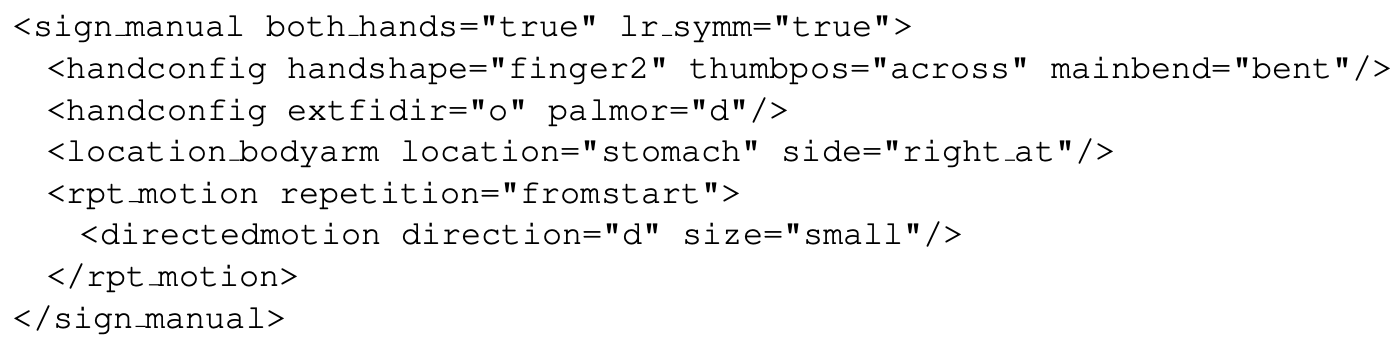
\includegraphics[width=\linewidth]{chap3/sigml-example.png} 
\caption{SiGML transcription of 'here'}
\label{fig-sigml}
\end{figure}

\begin{figure}[hbt!]
\center
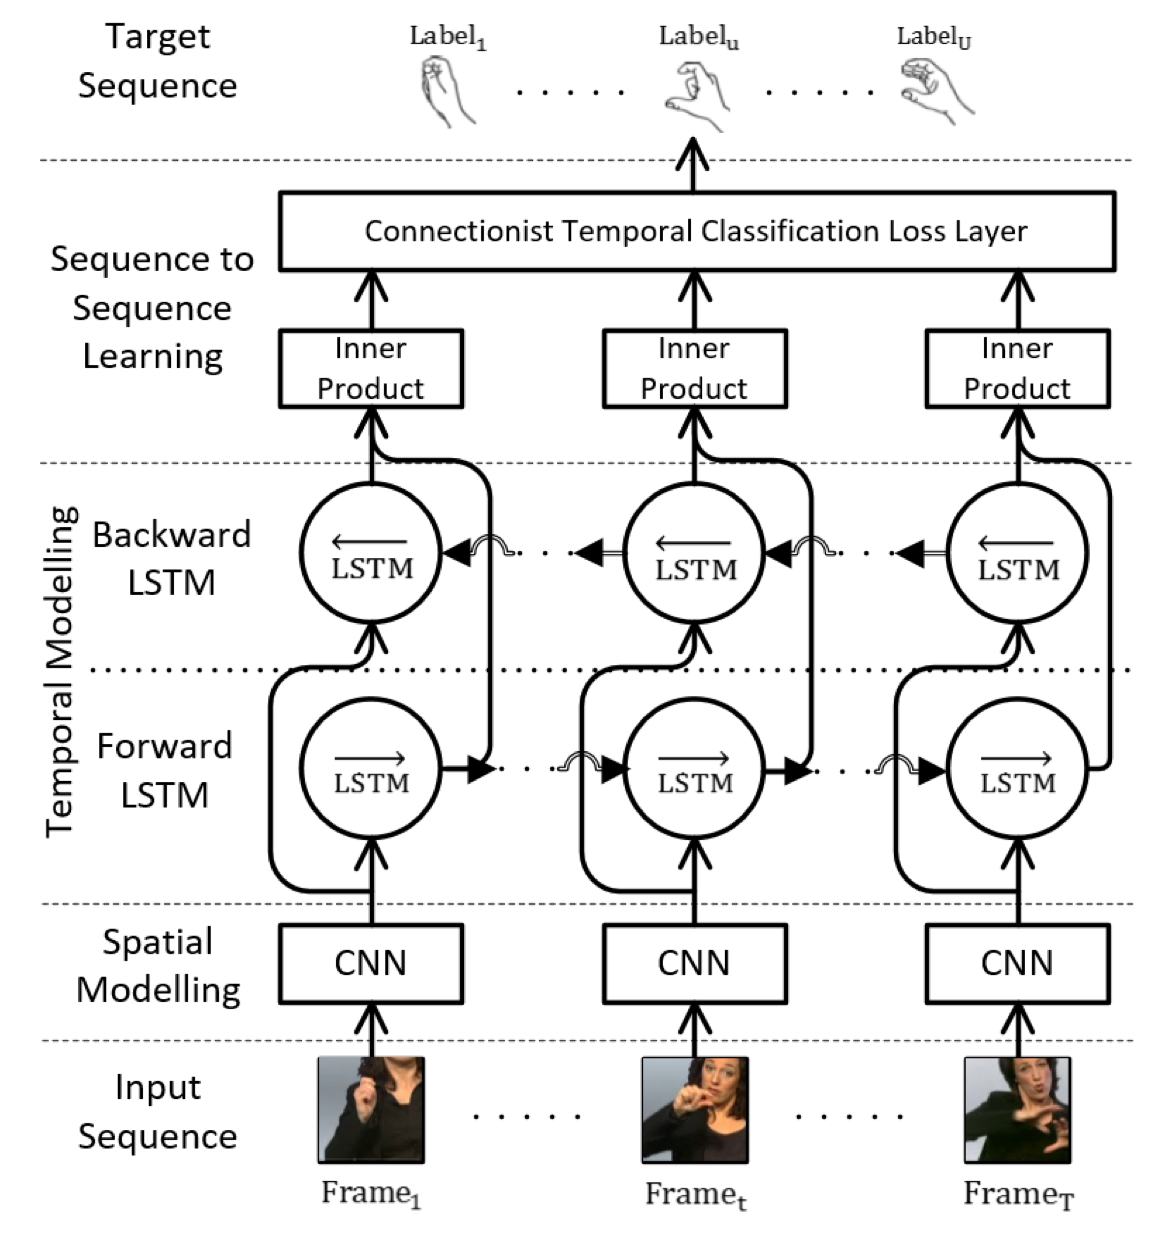
\includegraphics[width=\linewidth]{chap3/temporal-modeling.png} 
\caption{Temporal modeling using SubUNets}
\label{temporal-modeling}
\end{figure}

\begin{figure}[hbt!]
\center
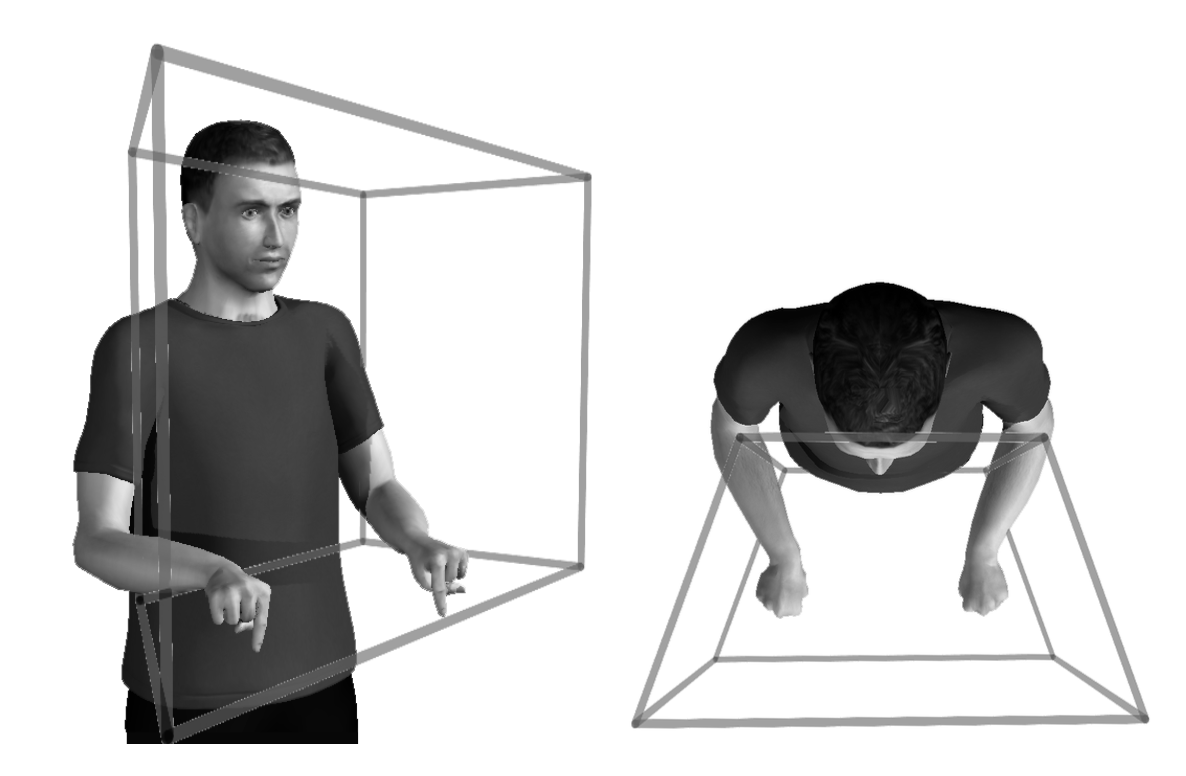
\includegraphics[width=\linewidth]{chap3/signing-space.png} 
\caption{Signing Space}
\label{fig-signing-space}
\end{figure}

\begin{figure}[hbt!]
\center
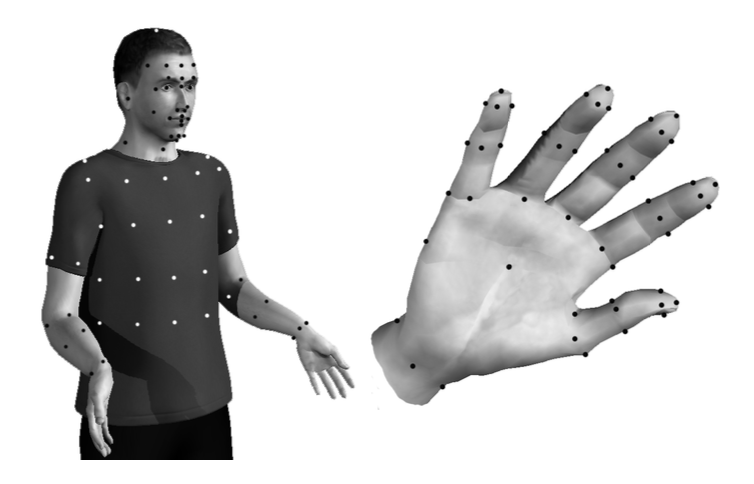
\includegraphics[width=\linewidth]{chap3/signing-locations.png} 
\caption{Signing Locations}
\label{fig-signing-locations}
\end{figure}

\begingroup
\footnotesize
\begin{landscape}
\begin{longtable}{|>{\hspace{0pt}}m{0.142\linewidth}|>{\hspace{0pt}}m{0.083\linewidth}|>{\hspace{0pt}}m{0.065\linewidth}|>{\hspace{0pt}}m{0.063\linewidth}|>{\hspace{0pt}}m{0.077\linewidth}|>{\hspace{0pt}}m{0.063\linewidth}|>{\hspace{0pt}}m{0.109\linewidth}|>{\hspace{0pt}}m{0.073\linewidth}|>{\hspace{0pt}}m{0.106\linewidth}|>{\hspace{0pt}}m{0.079\linewidth}|>{\hspace{0pt}}m{0.063\linewidth}|}
\caption{Public Available Large Scale Datasets}\\ 
\hline
\rowcolor[rgb]{0.753,0.753,0.753} DATASET & LANG & SIG\par{}NERS & CLA\par{}SSES & VIDEO \par{}INST. & DUR.~\par{}(H) & RES. & FPS & TYPE & MODA\par{}LITIES & YEAR \endfirsthead 
\hline
Signum SI & German & 25 & 780 & 19500 & 55.3 & 776x578 & 30 & continuous & RGB & 2007 \\ 
\hline
Signum isol. & German & 25 & 455 & 11375 & 8.43 & 776x578 & 30 & both & RGB & 2007 \\ 
\hline
Signum subset & German & 1 & 780 & 2340 & 4.92 & 776x578 & 30 & both & RGB & 2007 \\ 
\hline
Phoenix SD & German & 9 & 1231 & 6841 & 10.71 & 210x260 & 25 & continuous & RGB & 2014 \\ 
\hline
Phoenix SI & German & 9 & 1117 & 4667 & 7.28 & 210x260 & 25 & continuous & RGB & 2014 \\ 
\hline
CSL SD & Chinese & 50 & 178 & 25000 & 100+ & 1920x1080 & 30 & continuous & RGB+D & 2016 \\ 
\hline
CSL SI & Chinese & 50 & 178 & 25000 & 100+ & 1920x1080 & 30 & continuous & RGB+D & 2016 \\ 
\hline
CSL isol. & Chinese & 50 & 500 & 125000 & 67.75 & 1920x1080 & 30 & isolated & RGB+D & 2016 \\ 
\hline
Phoenix-T & German & 9 & 1231 & 8257 & 10.53 & 210x260 & 25 & continuous & RGB & 2018 \\ 
\hline
ASL 100 & English & 189 & 100 & 5736 & 5.55 & varying & varying & isolated & RGB & 2019 \\ 
\hline
ASL 1000 & English & 222 & 1000 & 25513 & 24.65 & varying & varying & isolated & RGB & 2019 \\ 
\hline
GSL isol. & Greek & 7 & 310 & 40785 & 6.44 & 848x480 & 30 & isolated & RGB+D & 2019 \\ 
\hline
GSL SD & Greek & 7 & 310 & 10290 & 9.59 & 848x480 & 30 & continuous & RGB+D & 2019 \\
\hline
\end{longtable}
\label{tab:public-large-datasets}
\end{landscape}

\endgroup 
%\input{MainText/chapter4} 
%\input{MainText/chapter5} 
 
%----------------------------------------------------------------------------------------
%	APPENDICES
%----------------------------------------------------------------------------------------

%\addtocontents{toc}{\vspace{2em}} % Add a gap in the Contents, for aesthetics
%\appendix % Starts of appendices
%
%\numberedchapter
%

\chapter{About Appendices} \label{appA}


Appendices are optional and should only be used if necessary.
%\input{MainText/appendixB}
%\input{MainText/appendixC}

%----------------------------------------------------------------------------------------
%	BIBLIOGRAPHY
%----------------------------------------------------------------------------------------

\addtocontents{toc}{\vspace{2em}} % Add a gap in the Contents, for aesthetics
\unnumberedchapter{Bibliography} % Title of the unnumbered chapter
\bibliography{Preamble/Thesis_bibliography} % The references information are stored in the file named "Thesis_bibliography.bib"


\end{document}  